~
\newpage
\section{Carbon Pricing \& Air Pollution Disparities in California}

\subsection{Empirical Strategy}

The goal of this chapter is to take the model of electricity generation and environmental inequality presented in Chapter 4 and apply it to simulate the effects of California's emissions trading scheme within the Western Interconnection. The proceeding sections will discuss the data the simulation uses and the results of the simulation. First though, this section will outline the approach I use to operationalize the model in Chapter 4. 



The central goal of this text is to analyze the effect of carbon pricing on environmental inequality, as measured by the environmental inequality gap (EI Gap) described in Chapter 4. To do so, the simulation model considers a set of policy scenarios with a range of carbon prices and measures the resulting disparities in air pollution under each policy scenario. Table \ref{policy_scenarios} outlines these different policy scenarios. For policy scenarios where all else is equal except the carbon price, the causal effect of the incremental change in the carbon price on the EI Gap is given by the difference the EI Gap between the two scenarios. 

Other than the carbon price itself, another relevant concern in the model is the presence of Border Carbon Adjustments (BCAs). Recall from section 2.5 that BCAs impose charges on imports or possibly rebates on exports of emissions intensive goods with the intention of preventing emissions leakage. The potential for carbon pricing to redistribute economic activity and the associated environmental consequences across jurisdictions is the primary motivation for creating a multi-region model of electricity generation in Chapter 4. Given the importance of these inter-regional dynamics in the model, the policy scenarios also vary in their use of BCAs. In the first five policy scenarios, there is no BCA; California power plants face a carbon price, but generation outside of California that is sold in California does not face a carbon price. In the final four policy scenarios, there is a uniform BCA. Under a uniform BCA, all of California's electricity imports face a uniform carbon price. The charge on electricity imports (\$/MWh) is the product of the domestic price of emissions (\$/tonne CO$_2$e) and the average emissions intensity of electricity (tonnes CO$_2$e/MWh) generated in the Western Interconnection outside of the California.\footnote{I recover the average emissions intensity of power generated in the Western Interconnection outside of California from the 2018 eGRID dataset.} Together, the nine policy scenarios enable the simulation to speak to the effect of carbon pricing on generation, greenhouse gas emissions, local air pollutant emissions, and disparities in local air pollutant emissions.

\begin{table}
    \centering
    \caption{Summary of Policy Scenarios \label{policy_scenarios}}
    \begin{tabular}{c c c}
        \hline\hline
        Policy Scenario & BCA? & Carbon Price (\$/tonne)\\
        \hline
        A & No & 0\\
        B & No & 20\\
        C & No & 40\\
        D & No & 60\\
        E & No & 80\\
        F & Yes & 20 \\
        G & Yes & 40 \\
        H & Yes & 60 \\
        I & Yes & 80 \\
    \hline    
    \end{tabular}
    \fignote[1]{Table summarizes the policy scenarios simulated. The Border Carbon Adjustment (BCA) in each scenario that uses a BCA is a uniform BCA, meaning that all electricity imports face a uniform carbon price. This carbon price is the average emissions intensity of all electricity generation in the exporting region times the domestic carbon price. In the actual implementation of the simulation model, there is an additional scenario that considers the situation where there would be a BCA but the carbon price is zero. This sceanrio is equivalent policy sceanrio A and is just used to help ensure the model functions properly. Each policy scenario is also re-considered under higher investment cost, a point addressed later in the section.
    }
\end{table}

With the policy scenarios established and provided all other necessary data is available, the simulation must just run the series of constrained optimizations laid out in the previous chapter. However, the size of this problem is prohibitive. There are 481 qualifying power plants in the Western Interconnection, each with four discrete choices (operate for California, operate of the Northwest, operate for the Southwest, and do not operate), meaning that solving the generation problem for a single hour with a given investment scenario would involve finding the least cost generation profile out of $4^{481}$ distinct generation profiles. This problem of course grows even larger when a large number of investment profiles and hourly demand schedules are under consideration. 

Following the standard approach in the literature for dealing with these prohibitively large optimization problems, I use $k$-means clustering to simplify the problem by forming representative powerplants and a representative demand schedule. 

Following the approach in \cite{fowlie2021border}, I use $k$-means clustering to group the hourly demand schedule into twenty-four clusters. This takes the three years of hourly electricity demand data from each region and parses it into a representative day. In some analyses, like analyzes concerned with a dynamic problem or performance under extreme situations, simplifying the demand schedule into a single day would not be desirable. In this case though, the analysis is primarily concerned with average outcomes that unfold over the course of a few years, so this strategy greatly reduces the computational burden of the model without any meaningful detriment to the interpretation of the results. 

Similarly, I use $k$-means clustering to cluster powerplants into generating groups. Because powerplants from different regions will differ in the carbon price they face, powerplants in each group must all be located in the same region. Similarly, because powerplants with different fuels will differ in the fuel prices they face, powerplants in each group must all use the same fuel. With these two boundaries set, I perform $k$-means clustering on all powerplants in a region based on their nameplate capacity and their heat rate. In each region, I create one group for coal powerplants, eight groups for gas powerplants, and one group for oil powerplants. Together, there are thirty powerplant groups, ten for each of the three regions. For each of these groups, I create a single representative powerplant, endowed with the total nameplate capacity and the average heat rate of all powerplants in the group. 

The generation optimization problem with these thirty representative powerplants is identical to the optimization in equation \ref{C_star}, with the one modification that in their implementation, representative powerplants have a continuous choice set. Let $q_{gtr}$ be the total generation of the powerplants in group $g$ at time $t$ for region $r$. Although $q_{itr}$ is discrete in Chapter 4, here $q_{gtr}$ is a continuous variable greater than zero, such that
\begin{equation}
    \sum_{r = 1}^3 q_{gtr} \leq 0.9 \cdot \overline{q_{gtr}},
\end{equation} 
where $\overline{q_{gtr}}$ is the sum of the nameplate capacities of all powerplants in group $g$. In practice, almost no powerplants have a capacity factor greater than 0.9, meaning that even the lowest cost powerplants are only able to run 90\% of their potential capacity. The constant $0.9$ in the capacity constraint above reflects this reality that powerplants cannot run at full capacity all the time, but must occasionally stop operating at operate at less than their maximum rated capacity. 

The results of the generation optimization for a given investment profile and demand schedule contain the total quantity of electricity generated by each of the thirty representative powerplants for each of the three regions. Ultimately though, the model must predict generation and emissions for individual powerplants. To compute the generation of individual powerplants from the generation of the representative powerplant groups, I start by summing the generation of each powerplant group across the three regions to find the total generation of the powerplants in the group during the given period. Using the total nameplate capacity of powerplants in the group, I calculate the capacity factor (actual generation/maximum possible generation) of each representative powerplant, and then assign this capacity factor to each powerplant in that group. For instance, suppose powerplant $i$ has a nameplate capacity of 100 MW and is in group $g$. If the total nameplate capacity of group $g$ is 1000 MW and the simulated generation of group $g$ in the period is 500 MW, then the capacity factor of group $g$ is 0.5. Then I compute the generation of powerplant $i$ as the product of the group $g$'s capacity factor and $i$'s nameplate capacity, 50 MW. This means that all powerplants in the same generation group end up with an identical distribution of capacity factors, but still vary in their total generation proportion to their nameplate capacity. 

To implement the investment optimization, I follow largely from \cite{weber2021dynamic}, and start by restricting the number of investment options of powerplants to a binary choice. Each powerplant can either make an investment to lower its heat rate by 1.5\% or not invest at all. Thirty powerplant groups is an acceptable number for the generation optimization, but because simulating a single investment scenario involves working through many the generation optimizations, thirty representative powerplants is too large for the investment optimization. To simplify this, I perform $k$-means clustering on the generation groups themselves, this time based only the average heat rate of the group, creating two clusters in California and two clusters outside of California.\footnote{Oil powerplants are excluded from the investment decision and are assumed to make heat rate improvements. These plants have unusually high heat rates and expensive fuels that would motivate investment. They make up a small share of all available generation, so this assumption does not have strong implications.} With four clusters that each make a binary choice, there are $2^4 = 16$ investment scenarios. Each investment scenario identifies which of the thirty representative groups of powerplants invests in a heat rate improvement that will reduce the generation group's average heat rate by 1.5\%. The optimization program loops through each of these sixteen investment scenarios and then reports the results of the investment scenario that had the least cost over the three year period. 

The investment cost function comes from \cite{weber2021dynamic}. Typically, the parameters of the investment cost function would need to be fit using a maximum likelihood estimation routine, but in this case, \cite{weber2021dynamic} has already estimated the parameters of this cost function. To complete the implementation of the investment decision model, I employ Weber's calibrated investment cost function. The powerplants Weber calibrates this investment cost function on are all gas powerplants in California, and it possible that these costs do not generalize easily to the wider variety of powerplants considered in this analysis. Later results suggest that these costs may be too low, so I also consider how investment decisions change when these investment costs are raised by an order of magnitude in Appendix A.5. 

Having simplified the set of investment decisions, the set of powerplants, and the set of demand profiles, I simulate the policy scenarios from Table \ref{policy_scenarios}. I implement the optimization program in Python using scipy.optimize.minimize, and let the initial point for each optimization be a vector of generation that corresponds to the situation where each representative powerplant produces just under 90\% of its capacity for domestic demand only. Using the technique previously described, these results for the generation of each group of powerplants is used to compute the generation for each individual powerplant for each representative hour. Annual generation totals are computed by taking the appropriate weights from each representative hour to form totals for a representative day, and multiplying by 365. Greenhouse gas emissions and local air pollutant emissions for each powerplant are calculated by multiplying the generation of each powerplant by the emissions intensities of each pollutant for each plant. 

While these powerplant-level predictions of generation and emissions are valuable, in it of themselves, they cannot speak to disparities in air pollution concentrations. The model in Chapter 4 builds the EI Gap by first designating communities as either ``Disadvantaged'' or ``Nondisadvantaged,'' a terminology that follows from California's SB 535. This bill requires that a proportion of the revenue raised through the state's emissions trading program go directly to projects in disadvantaged communities. To support this policy, California's EPA has developed a data-based approach to designating Census tracts as disadvantaged. Based on the technique California's EPA uses to determine the status of each Census tract in the state, I implement an analogous technique to determine the status of each Census tract in the Western Interconnection. 

Finally, I compute the EI Gap by summing the total emissions of a given local air pollutant in disadvantaged and nondisadvantaged Census tracts, dividing by their total areas, and then finding the difference between concentrations between disadvantaged and nondisadvantaged Census tracts. This is a suboptimal estimate for the pollution concentration, for the primary reason that air pollutants are not bound by Census tract boundaries. Ideally, this analysis might use a chemical dispersion model that would allow me to compute more detailed flows of emissions across the WECC. These models are again prohibitive and incorporating these is outside of the scope of these papers. The measure of concentrations used to form the EI Gap has its weaknesses, but ultimately the annual emissions of a given air pollutant per square mile provides an easy-to-interpret way these results. 


\subsection{Data}

All data sources I present in this section appear in Table \ref{data_sources} in Appendix A.5.

\subsubsection*{Generators}

Data on individual generators comes from the 2019 version of the Emissions \& Generation Resource Integrated Database (eGRID), a dataset released by the US Environmental Protection Agency (EPA). This dataset complies records on generator characteristics and generation collected through the US Energy Information Administration (EIA) Form EIA-923 and Form EIA-860 with emissions records collected by the EPA's Clean Air Markets Program. eGRID includes all generators at power plants in the US with a registered nameplate capacity, the maximum rated quantity of power a generator can create, of at least 1 MW.\footnote{For context, residential solar panels usually have a nameplate capacity somewhere between 1000 and 3000 W---meaning that the dataset covers all power plants that are at least 300 to 1000 times larger than residential rooftop solar.} At the generator level, this dataset provides key identifying characteristics of each generator including is primary fuel, its location, its age, its nameplate capacity, and whether or not it is operational. From this dataset of all utility-size generators, I filter out generators such that the final dataset includes only generators that were operational in 2019, are within the Western Interconnection, and use either coal, (natural) gas, or oil as their primary fuel. There are a handful of generators---two gas generators and thirteen oil generators---with negative heat rates that indicate the plant actually used more power in 2019 than it generated. Together these have a relatively small capacity of less than 75MW and their capacity factors (proportion of hours they are on) are near zero, meaning that excluding these generators will not influence the results in any meaningful way as they are almost never used and nearing retirement. 

\begin{figure}
    \centering
    \caption{Distribution of Generators by Region \& Fuel\label{generators_dist}}
    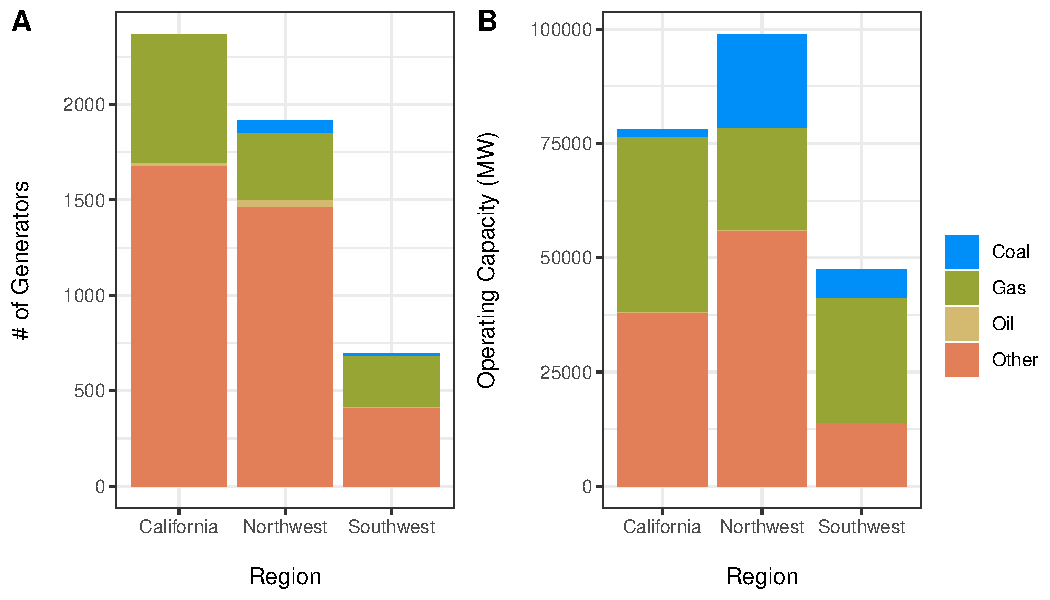
\includegraphics[width=\textwidth]{figures/chapter5_figures/regional_gens.pdf}
    \fignote[1]{
        Panel A breaks down generators by region and fuel type. Generators with fuel type `Other' are not included in the sample, but are displayed for reference on the overall distribution of generation in each region. The bulk of the `Other' fuels category is made up by renewable and nuclear generators. Generators vary substantially in their nameplate capacities, meaning that Panel A is not an accurate representation of the distribution of available capacity. By comparison, Panel B visualizes the distribution of generating capacity by region and fuel type. The relative size of the bars indicates that coal and natural gas generators have larger nameplate capacities than generators in the `Other' category. 
    }
\end{figure}

Figure \ref{generators_dist} displays the breakdown of generation across the three regions of the Western Interconnection, California, the Northwest, and the Southwest (see Figure \ref{wecc_regions} in Chapter 3 for a map of these regions). Panel A looks at all generators in across the regions, including those other than the coal, gas, and oil generators that this paper focuses on, for the purpose of comparison. Generators in this ``Other'' category (e.g., renewables and nuclear) account for the majority of generators in each region, and gas generators make up most of the remainder. California has more generators either the two regions, and almost has as many generators as the two other regions combined. While it is important to understand the distribution of the sample of generators, Panel A alone can be misleading as generators with different fuels often have substantially different capacities. Panel B displays the generating capacity of generators in each region by fuel type. Because renewable generators generally have nameplate capacities less than the average nameplate capacity of a generator in each region, then Panel B shows that generators in the `Other' category make up a smaller proportion of the total capacity than the proportion of total generators. On the other, coal generators are usually quite larger, so even though there are few coal generators visible in Panel A, coal generators account for a much larger share of generating capacity in Panel B. Additionally, although California has the most generators of the three regions, the Northwest has a greater generating capacity than California. 

eGRID reports emissions data at the power plant level but not the generator level, so for every generator, I assign it the emissions intensity and heat rate of the corresponding power plant. This treats generators within the same power plant as essentially homogenous with the exception of their nameplate capacities. Historically, eGRID has only reported data on the the emissions intensity of the greenhouse gas emissions of carbon dioxide (CO$_2$), methane (CH$_4$), and nitrous monoxide (N$_2$O), as well as local air pollutant emissions of nitrogen oxides (NO$_x$) and sulfur dioxide (SO$_2$).\footnote{Mercury emissions also appear in eGRID, but these are small enough that they are not worth including in this analysis.} The EPA recently released preliminary back estimates of fine particulate matter (PM2.5) emissions at the power plant level, and while these are not official estimates yet, I include these in the analysis. Using the global warming potentials in Table \ref{gwptable} in Chapter 2, I combine the emissions of individual greenhouse gases to measure all greenhouse gas emissions, measured in tonnes of carbon dioxide equivalent (CO$_2$e). 

\begin{figure}
    \centering
    \caption{Greenhouse Gas Emissions Intensities by Region \& Fuel \label{ghg_intensity}} 
    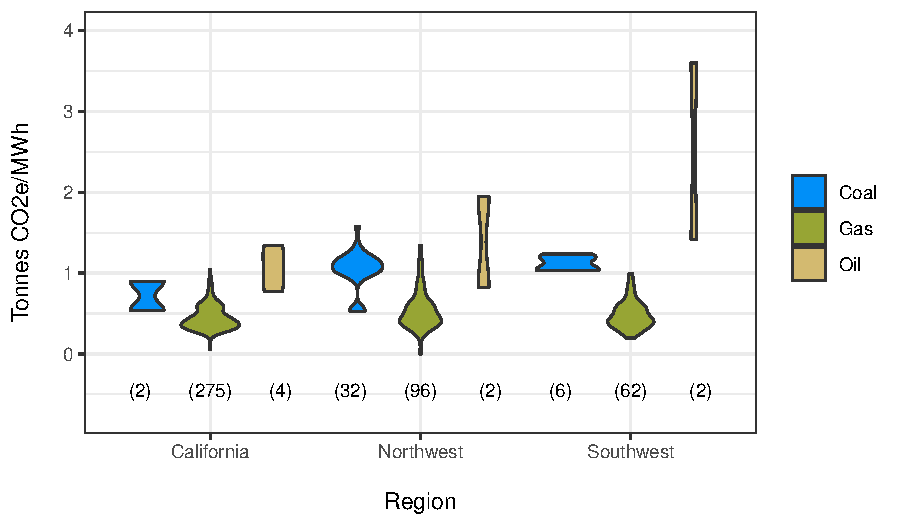
\includegraphics[width=\textwidth]{figures/chapter5_figures/EI_region_violin.pdf}
    \fignote[1]{
        Figure displays the distribution of greenhouse gas emissions intensities by region and fuel type. Emissions intensities are measured in tonnes of carbon dioxide equivalent (CO$_2$e) per megawatt-hour (MWh). For context, the average monthly US household electricity consumption was 0.886 MWh of electricity in 2021. The number of generators in group is displayed below the violinplot in parentheses. 
    }
\end{figure}

The violinplots in Figure \ref{ghg_intensity} display the distribution of greenhouse gas emissions intensities (CO$_2$e/MWh) by region and fuel. These emissions intensities are calculated by multiplying the emissions intensity of the specific variety of fuel a generator uses, measured in CO$_2$e/mmBTU, and multiplying it by the generator's heat rate, measured in mmBTU/MWh. The number of generators in each region and with each fuel is below the violinplot in parentheses. Overall, this shows that gas generators generally have the lowest greenhouse gas emissions intensities. In both the Northwest and Southwest, gas generators are almost always less emissions intensive than coal and oil generators. In California, coal, gas, and oil generators have similar emissions intensities, likely a result of regulation that has forced the closure of less efficient coal and oil power plants. Oil generators in general have the greatest spread in emissions intensities. 

\begin{figure}
    \centering
    \caption{Local Air Pollutant Emissions Intensities by Fuel\label{pol_intensities}}
    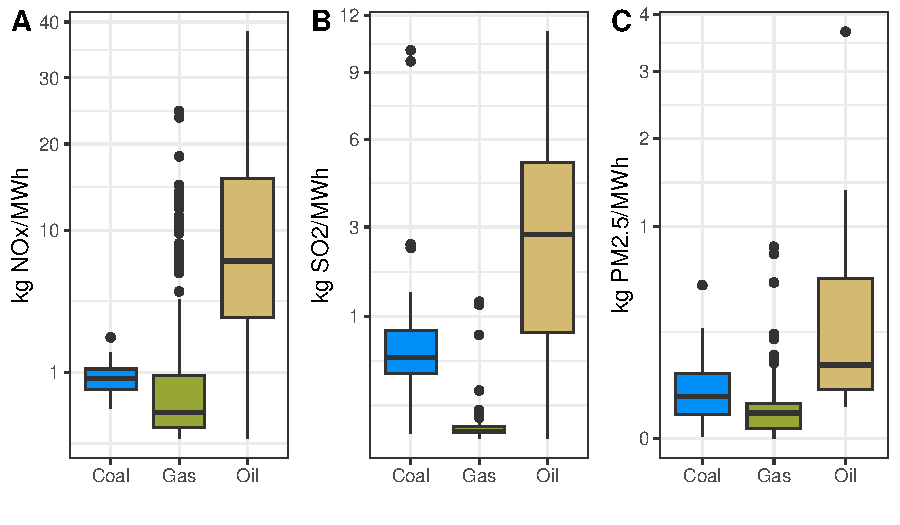
\includegraphics[width=\textwidth]{figures/chapter5_figures/local_poll_EI.pdf}
    \fignote[1]{
        Figure displays the distribution of criteria air pollutant emissions intensities by generator fuel type. Panel A, B, and C visualize these the distributions of nitrogen oxides (NO$_x$), sulfur dioxide (SO$_2$), and fine particulate matter (PM2.5). These distributions are highly right skewed, so the vertical axis in each panel uses a squareroot transformation. 
    }
\end{figure}

Figure \ref{ghg_intensity} demonstrates that while there is some variation in the greenhouse gas emissions intensities of generators across the different regions and fuels, these distributions are fairly close to each other. This is not the case for local air pollutant emissions intensities. Figure \ref{pol_intensities} displays these distributions for each of the three local air pollutants, NO$_x$, SO$_2$, and PM2.5, for generators of each fuel category. First note that all figures use a squareroot scale on the vertical axis so these distributions are clearer to see. For each pollutant, gas generators have the lowest median emissions intensity, coal the second lowest, and oil highest. Gas generators create essentially no SO$_2$ emissions, but it is not uncommon for gas generators to have just as high NO$_2$ emissions intensities as coal generators. Oil generators are again highly variable, sometimes varying my an order of magnitude. 

Lastly, I augment the generator data with data on the fuel prices of each type of generator. Power plants report their fuel costs on a regular basis (frequency depends on the fuel) as a part of Form EIA-860. The EIA reports these prices at the state level, so I aggregate these to get region-specific prices for coal and gas for power plants. There are so few power plants that continue to fuel oil that the EIA does not report the prices these power plants pay for fuel oil for data confidentiality. Instead, I use the price of West Texas Intermediate Crude oil out of Cushing, Oklahoma (the standard quote price for oil) reported by the EIA. The analysis will use time-invariant fuel prices, so I average prices over the relevant timeframe, and make the necessary conversions to get the price of each generator pays for fuel in USD/mmBTU. Additional details on the fuel prices appear in Appendix A.5 with Figures and Table \ref{fuel_prices}.

\begin{table}
    \centering
    \caption{Generator Summary Statistics}
\begin{tabular}{l c c c c c}
    \hline\hline
    Variable & Mean & St. Dev. & Min & Median & Max \\
    \hline\\[-1.8ex]
    \textit{Coal} \\
    \hline
    Generator Age (years) & 39.890 & 14.530 & 8 & 40.5 & 72 \\ 
Capacity Factor & 0.585 & 0.175 & 0.053 & 0.598 & 0.995 \\ 
Capacity (MW) & 340.704 & 261.183 & 1.500 & 363.500 & 856.800 \\ 
Heat Rate (mmBTU/MWh) & 10.066 & 2.492 & 5.534 & 10.736 & 16.158 \\ 
Input Price (\$/MWh) & 21.093 & 6.362 & 10.615 & 21.302 & 37.285 \\ 
tonnes CO$_2$e/MWh & 0.972 & 0.245 & 0.527 & 1.048 & 1.580 \\ 
kg NO$_x$/MWh & 0.852 & 0.372 & 0.210 & 0.801 & 2.344 \\ 
kg SO$_2$/MWh & 0.826 & 1.678 & 0.001 & 0.397 & 10.109 \\ 
kg PM2.5/MWh & 0.067 & 0.075 & 0.0001 & 0.043 & 0.522 \\ \\[-1.8ex]
\textit{Gas} \\
\hline
Generator Age (years) & 18.663 & 13.438 & 0 & 16 & 71 \\ 
Capacity Factor & 0.292 & 0.283 & 0.000 & 0.205 & 1.000 \\ 
Capacity (MW) & 67.707 & 84.937 & 0.100 & 40.000 & 806.000 \\ 
Heat Rate (mmBTU/MWh) & 9.050 & 3.049 & 1.033 & 8.784 & 22.107 \\ 
Input Price (\$/MWh) & 43.766 & 15.554 & 5.517 & 40.805 & 105.106 \\ 
tonnes CO$_2$e/MWh & 0.482 & 0.163 & 0.055 & 0.466 & 1.173 \\ 
kg NO$_x$/MWh & 2.479 & 4.657 & 0.000 & 0.223 & 24.725 \\ 
kg SO$_2$/MWh & 0.035 & 0.186 & 0.000 & 0.003 & 2.191 \\ 
kg PM2.5/MWh & 0.046 & 0.187 & 0.000 & 0.014 & 1.367 \\ \\[-1.8ex]
\textit{Oil} \\
\hline
Generator Age (years) & 32.147 & 18.007 & 6 & 37.5 & 61 \\ 
Capacity Factor & 0.099 & 0.185 & 0.000 & 0.002 & 0.772 \\ 
Capacity (MW) & 17.941 & 27.051 & 1.000 & 2.500 & 74.500 \\ 
Heat Rate (mmBTU/MWh) & 16.243 & 8.641 & 7.234 & 15.985 & 48.441 \\ 
Input Price (\$/MWh) & 186.250 & 99.084 & 82.945 & 183.291 & 555.443 \\ 
tonnes CO$_2$e/MWh & 1.219 & 0.632 & 0.538 & 1.173 & 3.600 \\ 
kg NO$_x$/MWh & 12.710 & 13.192 & 0.000 & 7.257 & 38.160 \\ 
kg SO$_2$/MWh & 1.732 & 2.410 & 0.000 & 1.225 & 11.101 \\ 
kg PM2.5/MWh & 1.000 & 1.354 & 0.018 & 0.121 & 3.682 \\ \\[-1.8ex]
\hline \\[-1.8ex] 
\end{tabular}
\fignote[1]{$N_\text{Coal} = 100$, $N_\text{Gas} = 1267$, $N_\text{Oil} = 34$}
\end{table}



\subsubsection*{Electricity Demand}


\subsubsection*{Disadvantaged Communities}

\begin{figure}
    \centering
    \caption{Disadvantaged Communities (DACs) Designation Comparison}
    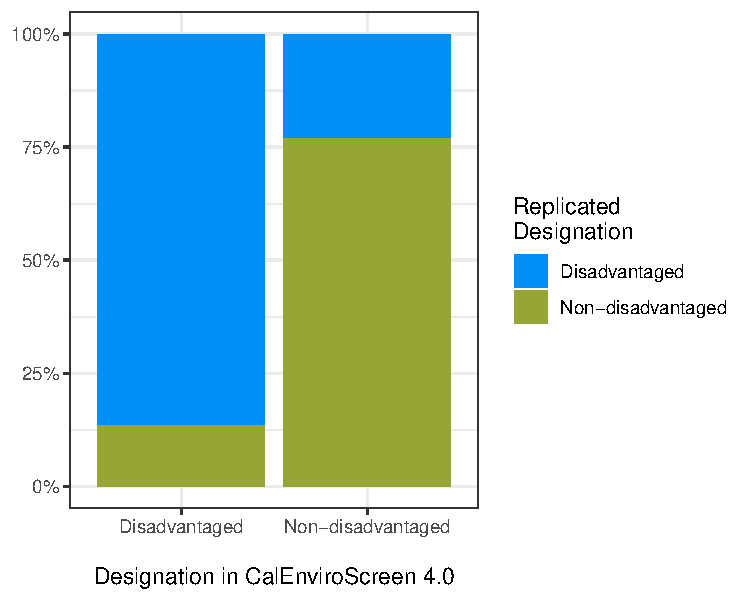
\includegraphics[width=0.7\textwidth]{figures/chapter5_figures/DAC_designation.pdf}
    \fignote[.9]{
        Figure shows\ldots
    }
\end{figure}

\subsection{Results}

\subsubsection*{Generation}



\subsubsection*{Greenhouse Gas Emissions}



\subsubsection*{Local Air Pollution Emissions}



\subsubsection*{The Environmental Inequality Gap}

\begin{figure}
    \centering
    \caption{The EI Gap for NO$_x$}
    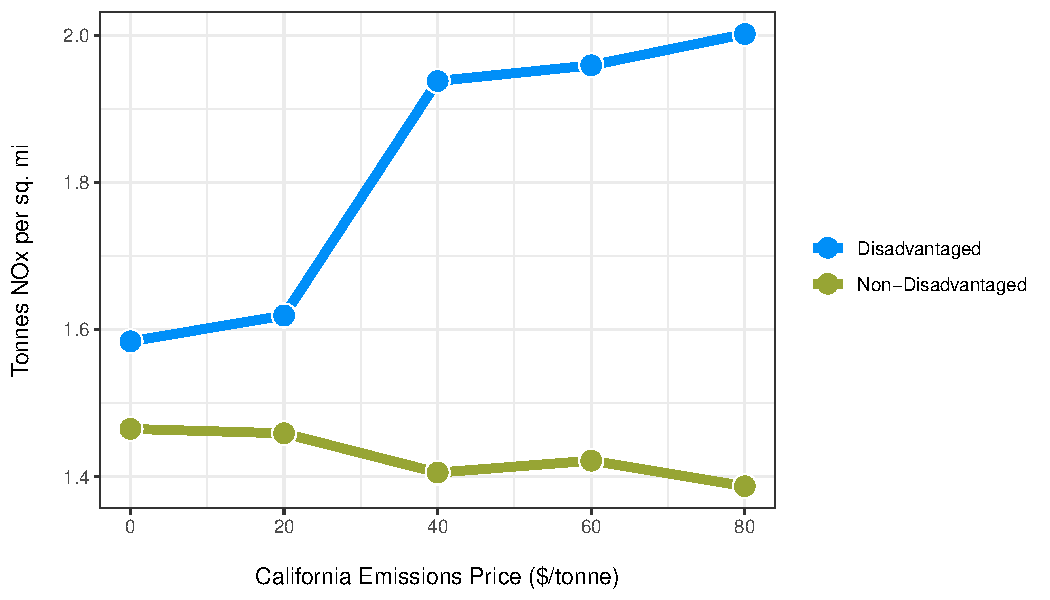
\includegraphics[width=\textwidth]{figures/chapter5_figures/ei_gap_bca_nox.pdf}
    \fignote[1]{
        Figure shows\ldots
    }
\end{figure}

\begin{figure}
    \centering
    \caption{The EI Gap for NO$_x$ in California}
    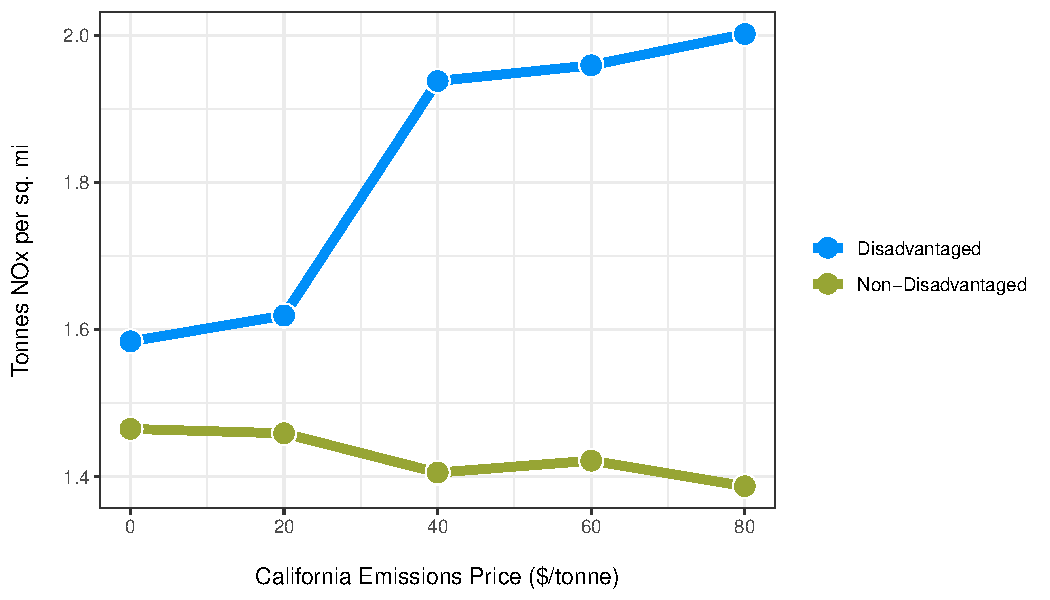
\includegraphics[width=\textwidth]{figures/chapter5_figures/ei_gap_bca_nox.pdf}
    \fignote[1]{
        Figure shows\ldots
    }
\end{figure}




\subsection{Diagnostics}





